
%\section{Extensions}

%%%%%%%%%%%%%%%%%%%%%%%%%%%
%%%%%%%%%%%%%%%%%%%%%%%%%%%
%%%%%%%%%%%%%%%%%%%%%%%%%%%
\section{Left, right and full graph joins.}\label{sec:leftrightfull}
\begin{figure*}
	\centering
	\begin{minipage}[t]{0.3\textwidth}
		\centering
		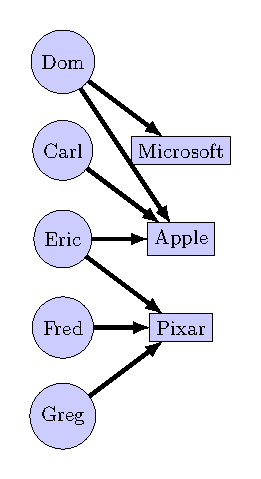
\includegraphics[scale=.6]{fig/03joins/aaa_left_affiliation}
		\subcaption{Company Membership, Graph $\mathcal{A}$}
		\label{fig:companymembership}
	\end{minipage}\quad
	\begin{minipage}[t]{0.3\textwidth}
		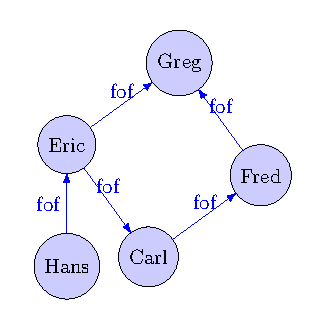
\includegraphics[scale=.6]{fig/03joins/aaa_left_users2}
		\subcaption{Social Network Friendship, Graph $\mathcal{N}$}
		\label{fig:osnforleftjoin}
	\end{minipage}\quad
	\begin{minipage}[t]{0.3\textwidth}
		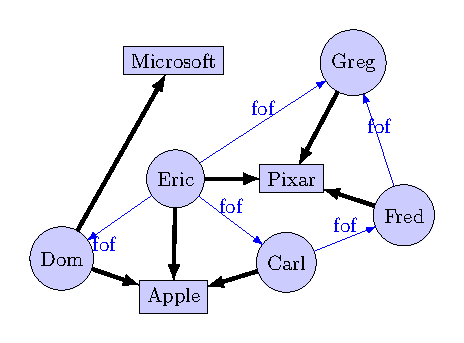
\includegraphics[scale=.6]{fig/03joins/aaa_left_merged2_prev}
		\subcaption{Merged Graph, $\mathcal{A}\;\leftouterjoin_{\;\sim}^\vee\;\mathcal{N}$}
		\label{fig:leftjoindesiredsol}
	\end{minipage}
\end{figure*}
The following example motivates the need of an extension of the aforementioned graph operators, since they cannot describe all the possible join combinations for graphs.

\begin{example}
	Suppose to have a company membership bipartite graph $\mathcal{A}$ (Figure \ref{fig:companymembership}), where each employee is associated to a company where (s)he works. Suppose now to have another graph $\mathcal{N}$ (Figure \ref{fig:osnforleftjoin}) providing a social network where some users are provided. Given that we can infer a predicate $\sim$ which finds correspondences between each employee in $\mathcal{A}$ and their on-line account in $\mathcal{N}$, join the graphs so that $\mathcal{A}$ is enriched with the friendship edges from $\mathcal{N}$ as in Figure \ref{fig:leftjoindesiredsol}. For this toy example, such $\sim$ function associates the employee and the social network users that have the same name.
	\medskip
	

	Concerning the edges, we must adopt a disjunctive semantics, because the edges in $\mathcal{A}$ link employees to companies, while the ones in $\mathcal{N}$ link friends among them. As a consequence, such edges could never match with a conjunctive semantics: in order to preserve the \texttt{worksFor} relationships in $\mathcal{A}$ and inherit the friendship relationships \texttt{fof} among employees, we must adopt the disjunctive semantics.
	
	Concerning the vertices that have to be returned by the graph join operation, we can observe that graph $\mathcal{N}$ contains more users than the employees in $\mathcal{A}$, and that $\mathcal{A}$ contains employees that have no account in $\mathcal{N}$. Since is $\mathcal{A}$ the graph to be enriched, we want to preserve all the information in $\mathcal{A}$ and to discard all the users in $\mathcal{N}$. We can even observe that the companies are not included in the definition of $\sim$, and hence a $V_{\mathcal{A}}\bowtie_\sim V_{\mathcal{N}}$ between the vertices shall not return any company. For this reason, we have to perform the left join $V_{\mathcal{A}}\leftouterjoin_\sim V_{\mathcal{N}}$ over the vertices, so that all the employees and the companies from graph $\mathcal{A}$ are preserved, while the users in  $\mathcal{N}$ that are not employees are not represented in the final graph. 
\end{example}



We must observe that the operation outlined by the previous example is not matched by the former definitions of graph joins.
Consequently, we now introduce the outer join operators by extending the join's vertex definition: if we want to
include only the unmatched vertices belonging to the left join operand then we have a \textbf{left  join} ($\leftouterjoin$), which is defined as follows:

\begin{definition}[Graph Left  $\theta$-Join]\label{def:leftjoin}
	\label{def:graphleftjoin} \index{product, $\otimes_\theta$!for property graphs!left join}
	Given two graphs $G_a=(V,E,A_v,A_e)$ and $G_b=(V',E',A_v',A_e')$, a \textbf{graph left
		$\theta$-join} is defined by extension of Definition \ref{def:graphjoin} as follows:
	\begin{equation*}
	G_a\leftouterjoin_\theta^{\textbf{\textup{es}}} G_b=(V\leftouterjoin_\theta V',E_{\textup{\textbf{es}}},A_v\cup A_v',A_e\cup A_e')
	\end{equation*}
	where $\leftouterjoin_\theta$ the left outer $\theta$-join  among the vertices.
\end{definition}

If we  symmetrically include only the vertices from the right graph then we have a \textbf{right  join} ($\rightouterjoin$), and thus the following definition can be provided:

\begin{definition}[Graph Right $\theta$-Join]\label{def:rightjoin}
	\label{def:graphrightjoin} \index{product, $\otimes_\theta$!for property graphs!right join}
	Given two graphs $G_a=(V,E,A_v,A_e)$ and $G_b=(V',E',A_v',A_e')$, a \textbf{graph right
		$\theta$-join} is defined as:
	\begin{equation*}
	G_a\rightouterjoin_\theta^{\textbf{\textup{es}}} G_b=(V\rightouterjoin_\theta V',E_{\textup{\textbf{es}}},A_v\cup A_v',A_e\cup A_e')
	\end{equation*}
	where $\rightouterjoin_\theta$ the right outer $\theta$-join  among the vertices.
\end{definition}

Given that both the conjunctive and the disjunctive semantics are expressible as joins among the edges and given the well known  properties for the relational algebra operators, we have that for \textbf{es}$=\wedge$ or \textbf{es}$=\vee$ the following rewriting rule follows:

\[G_a\rightouterjoin_\theta^{\textbf{\textup{es}}} G_b = G_b\leftouterjoin_\theta^{\textbf{\textup{es}}} G_a\]

If we want also to include
the excluded vertices from both graphs we have a \textbf{full join} \index{product, $\otimes_\theta$!for property graphs!full join} ($\fullouterjoin$). Similarly to the graph right $\theta$-join, we can define this new operator either as a graph join where the vertices undergo a full $\theta$-join or as a composition of the left and right join as follows when \textbf{es} is one of the two aforementioned edge semantics:

\[G_a\fullouterjoin_\theta^{\textbf{\textup{es}}} G_b = G_a\rightouterjoin_\theta^{\textbf{\textup{es}}} G_b \cup G_a\leftouterjoin_\theta^{\textbf{\textup{es}}} G_b\]

As a consequence, we can say that the graph joins are a class of join operators, where an arbitrary combination $\otimes$ of vertices and \textbf{es} of edges is provided. Consequently, we can provide the following definition including all the previously defined graph join operators.

\begin{definition}[Graph $\otimes_\theta$ product]\label{def:otimesjoin}
	\label{def:graphrightjointmes}\index{product, $\otimes_\theta$!for property graphs}
	Given two graphs $G_a=(V,E,A_v,A_e)$ and $G_b=(V',E',A_v',A_e')$, the class of all the possible graph join operators is defined by the following \textbf{graph $\otimes_\theta$ product}:
	\begin{equation*}
	G_a\otimes_\theta^{\textbf{\textup{es}}} G_b=(V\otimes_\theta V',E_{\textup{\textbf{es}}},A_v\cup A_v',A_e\cup A_e')
	\end{equation*}
	where $\otimes_\theta$ is an arbitrary $\theta$-join operation among the vertices.
\end{definition}

%Figure \vref{fig:conjdisjbasicexouter} already provided an example of all the previously described examples of outer joins with a disjunctive semantics.

\begin{figure}[!ph]
	\centering
	\begin{adjustbox}{max width=\textwidth}
		\begin{minipage}[b]{.25\textwidth}
			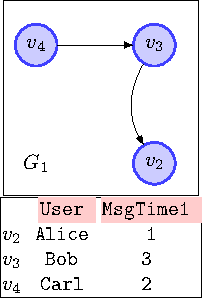
\includegraphics[scale=0.8]{fig/03joins/g1_mod_tab.pdf}
			\subcaption{$G_1$}\label{fig:figjoing1bisa}
		\end{minipage}
		\begin{minipage}[b]{.25\textwidth}
			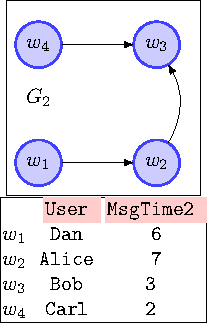
\includegraphics[scale=0.8]{fig/03joins/g2_mod_tab}
			\subcaption{$G_2$}\label{fig:figjoing2bis}
		\end{minipage}
	\end{adjustbox}\\
	\begin{minipage}[b]{.3\linewidth}
		\centering
		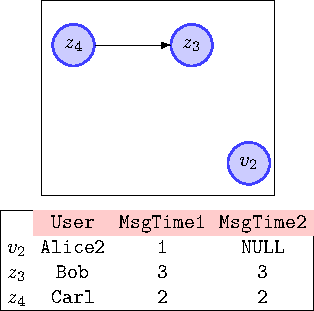
\includegraphics[scale=0.8]{fig/03joins/cong_left}
		\subcaption{$G_1\leftouterjoin_{\theta}^\wedge G_2$}\label{fig:conj_left}
	\end{minipage}
	\begin{minipage}[b]{.35\linewidth}
		\centering
		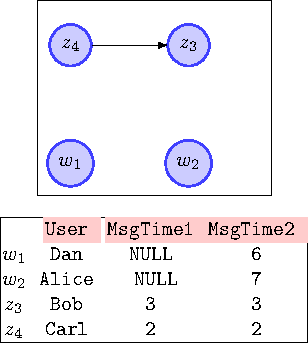
\includegraphics[scale=0.8]{fig/03joins/cong_right}
		\subcaption{$G_1\rightouterjoin_{\theta}^\wedge G_2$}\label{fig:conj_right}
	\end{minipage}
	\begin{minipage}[b]{.3\linewidth}
		\centering
		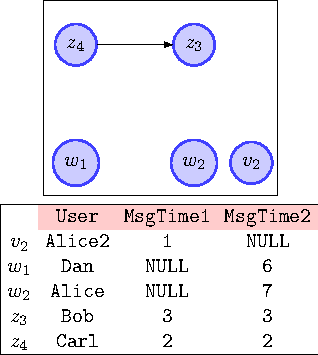
\includegraphics[scale=0.8]{fig/03joins/cong_both}
		\subcaption{$G_1\fullouterjoin_{\theta}^\wedge G_2$}\label{fig:conj_both}
	\end{minipage}
	\begin{minipage}[b]{.3\linewidth}
		\centering
		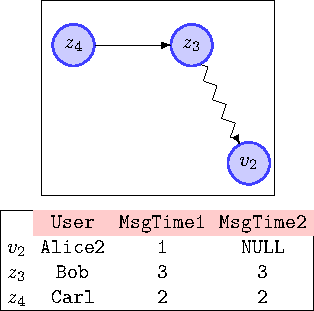
\includegraphics[scale=0.8]{fig/03joins/disj_left}
		\subcaption{$G_1\leftouterjoin_{\theta}^{\vee} G_2$}\label{fig:disj_left}
	\end{minipage}
	\begin{minipage}[b]{.3\linewidth}
		\centering
		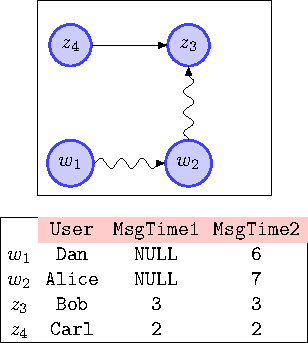
\includegraphics[scale=0.8]{fig/03joins/disj_right}
		\subcaption{$G_1\rightouterjoin_{\theta}^{\vee} G_2$}\label{fig:disj_right}
	\end{minipage}
	\begin{minipage}[b]{.35\linewidth}
		\centering
		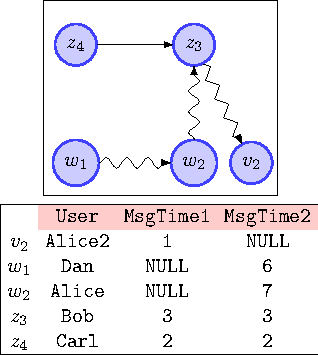
\includegraphics[scale=0.8]{fig/03joins/disj_both}
		\subcaption{$G_1\fullouterjoin_{\theta}^{\vee} G_2$}\label{fig:disj_both}
	\end{minipage}
	\begin{minipage}[b]{.3\linewidth}
		\centering
		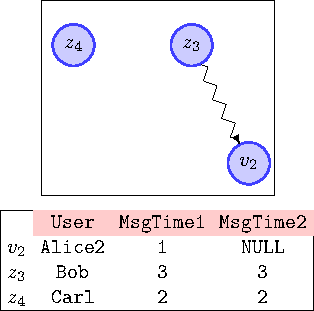
\includegraphics[scale=0.8]{fig/03joins/diff_left}
		\subcaption{$G_1\leftouterjoin_{\theta}^{\delta\vee} G_2$}\label{fig:diff_left}
	\end{minipage}
	\begin{minipage}[b]{.3\linewidth}
		\centering
		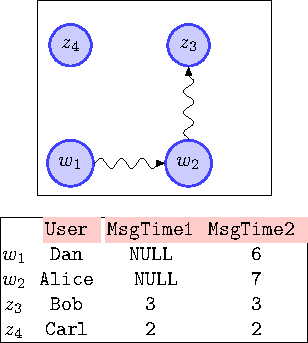
\includegraphics[scale=0.8]{fig/03joins/diff_right}
		\subcaption{$G_1\rightouterjoin_{\theta}^{\delta\vee} G_2$}\label{fig:diff_right}
	\end{minipage}
	\begin{minipage}[b]{.35\linewidth}
		\centering
		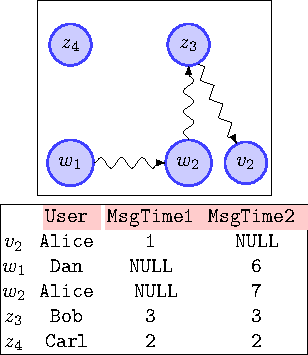
\includegraphics[scale=0.8]{fig/03joins/diff_both}
		\subcaption{$G_1\fullouterjoin_{\theta}^{\delta\vee} G_2$}\label{fig:diff_both}
	\end{minipage}
	\caption{Representation of outer joins over both conjunctive and disjunctive joins, where $\theta$ is defined as
		\texttt{MsgTime2$\leq$MsgTime1}. Wiggled edges represent the edges obtained from right graph while zigzag edges represent the ones from left one. Straight-lined edges are
		the ones provided by the definition of the conjunctive join, and hence $E_{\Join}$. \texttt{NULL} values only
		appear in the tabular representation, while the provided vertex merge definition do not insert null values}
	\label{fig:dataexampleouters}
\end{figure}

\begin{example}
As a further example, let us take a look at Figure \ref{fig:dataexampleouters}: suppose to have two graphs $G_1$ (\subref{fig:figjoing1bisa}) and $G_2$ (\subref{fig:figjoing2bis}), describing interaction graphs between some users within different social network: any edge $u\xrightarrow{\delta}v$ describes that a user $u.\texttt{User}$ sent a message to $v.\texttt{User}$ at a time $u.\texttt{MsgTime}_i$, that received it and read it at time $v.\texttt{MsgTime}_i$. Given a predicate $\theta$ allowing to match the same users within different networks, we want to show which is the meaning of the different graph joins on top of these data structures.

Generally speaking, the graph conjunctive semantics is used to retrieve the interactions occurring in different networks between the same users, even if at different times. The usage of the left (\subref{fig:conj_left}), right (\subref{fig:conj_right}) or full join (\subref{fig:conj_both}) could be used to only change the result set of the vertices. Moreover, on all the three different cases of graph joins, the conjunctive semantics does not change the edges that are returned in the final result, since that semantics imply that the edges must appear in both graphs among the matched vertices.

As a consequence, the outer joins over the disjunctive semantics allow to return also the interactions coming either from the left operand (\subref{fig:disj_left}), or from the right one (\subref{fig:disj_right}) or both (\subref{fig:disj_both}).

As a last step, we would like to intercept the interaction that only appear either in the left graph, or in the right one, or the interaction occurring either in the left graph or in the right one but not in both. In order to do so, we can define another edge semantics $\delta\vee$, removing from the disjunctive semantics the edges that appear in the conjunctive semantics, that is:
\[E_{\delta\vee}=E_\vee\backslash E_\wedge\]
After this step, we can finally obtain the graphs depicted in Figures \ref{fig:diff_left}, \ref{fig:diff_right} and \ref{fig:diff_both}. 
\end{example}

As a final example, we want to show how graph full joins may help in the creation of a common schema, generated from the two graph sources' schemas, thus showing how graph joins can be used for at both the data ($D$) and model (or schema, $M$) level. 


\begin{figure}
	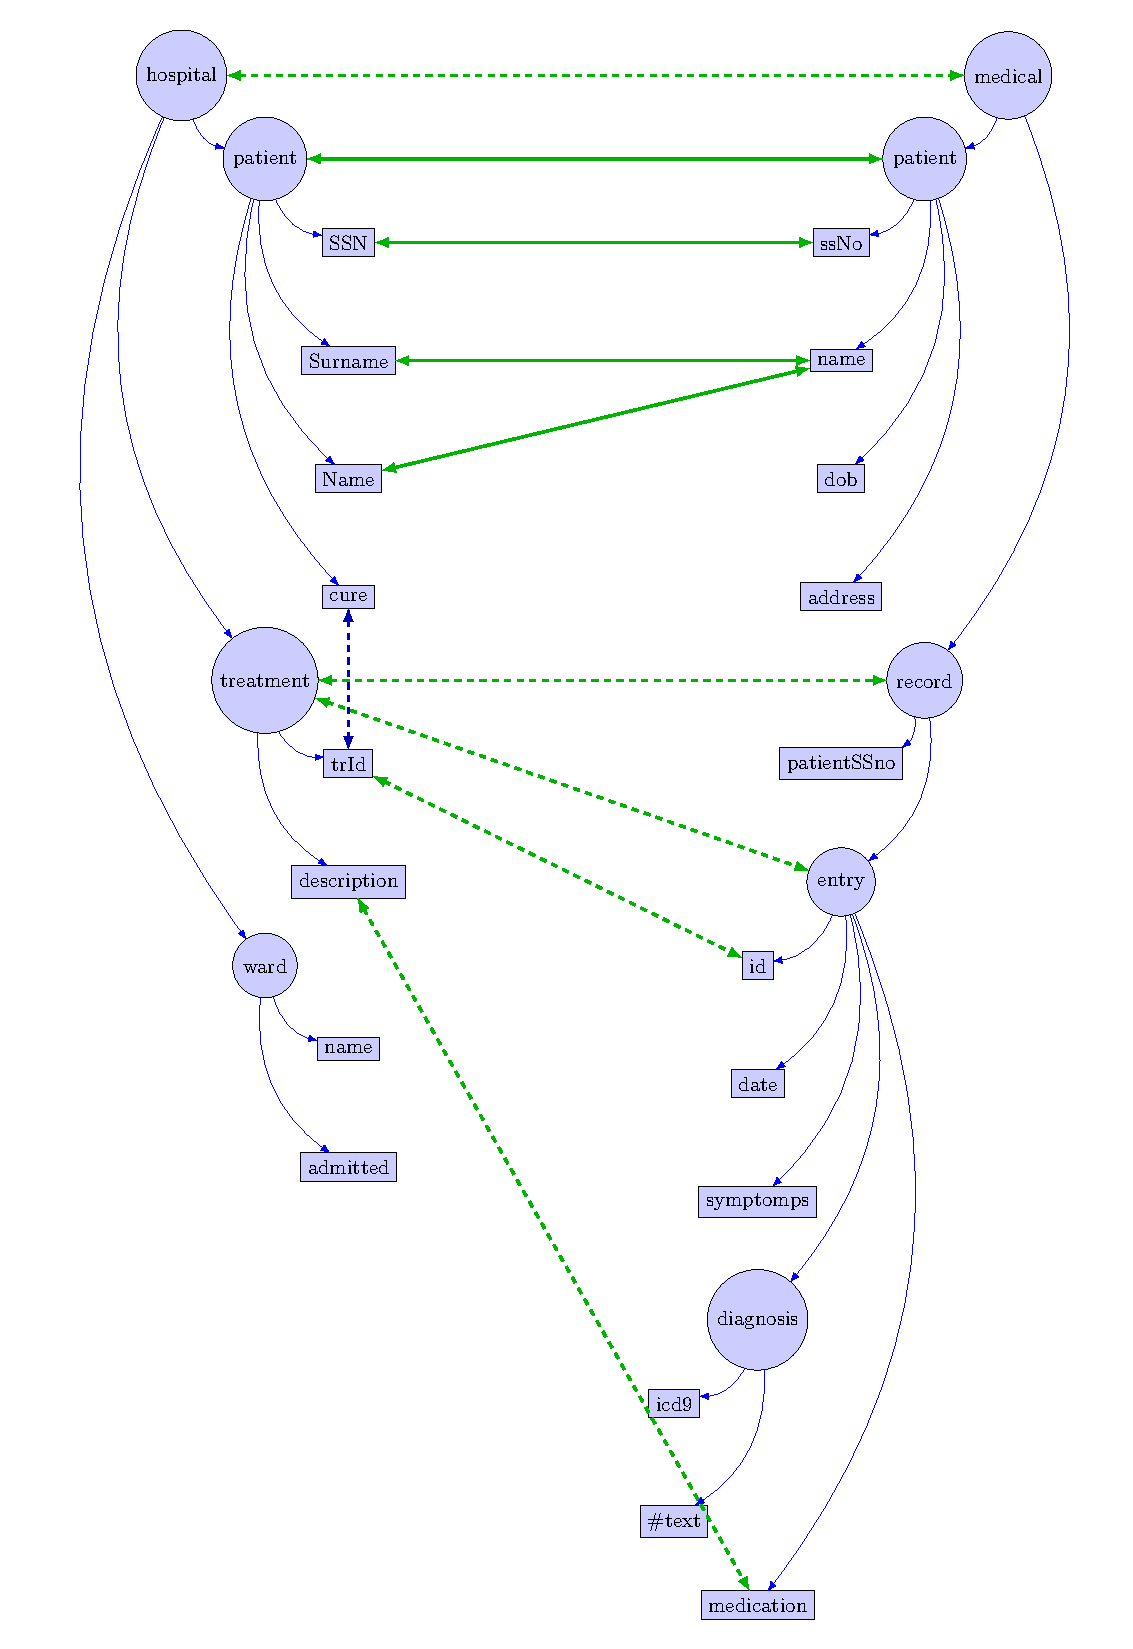
\includegraphics[width=\textwidth]{fig/03joins/ontologyLeftRight}
	\caption{Representing the containments in Figure \vref{fig:XMLAlignment} as the ontology graphs presented in \cite{euzenat2013d}: the left and the right graphs represent different schemas, where their blue edges express the containment relations. Green edges express either directly the result of the ontology alignment operation (continuous lines) or their refinements (dashed lines) that are going to be used to provide the integrated schema as a $\theta$ predicate.}
	\label{fig:semistructAsGraphCont}
\end{figure}\begin{figure}
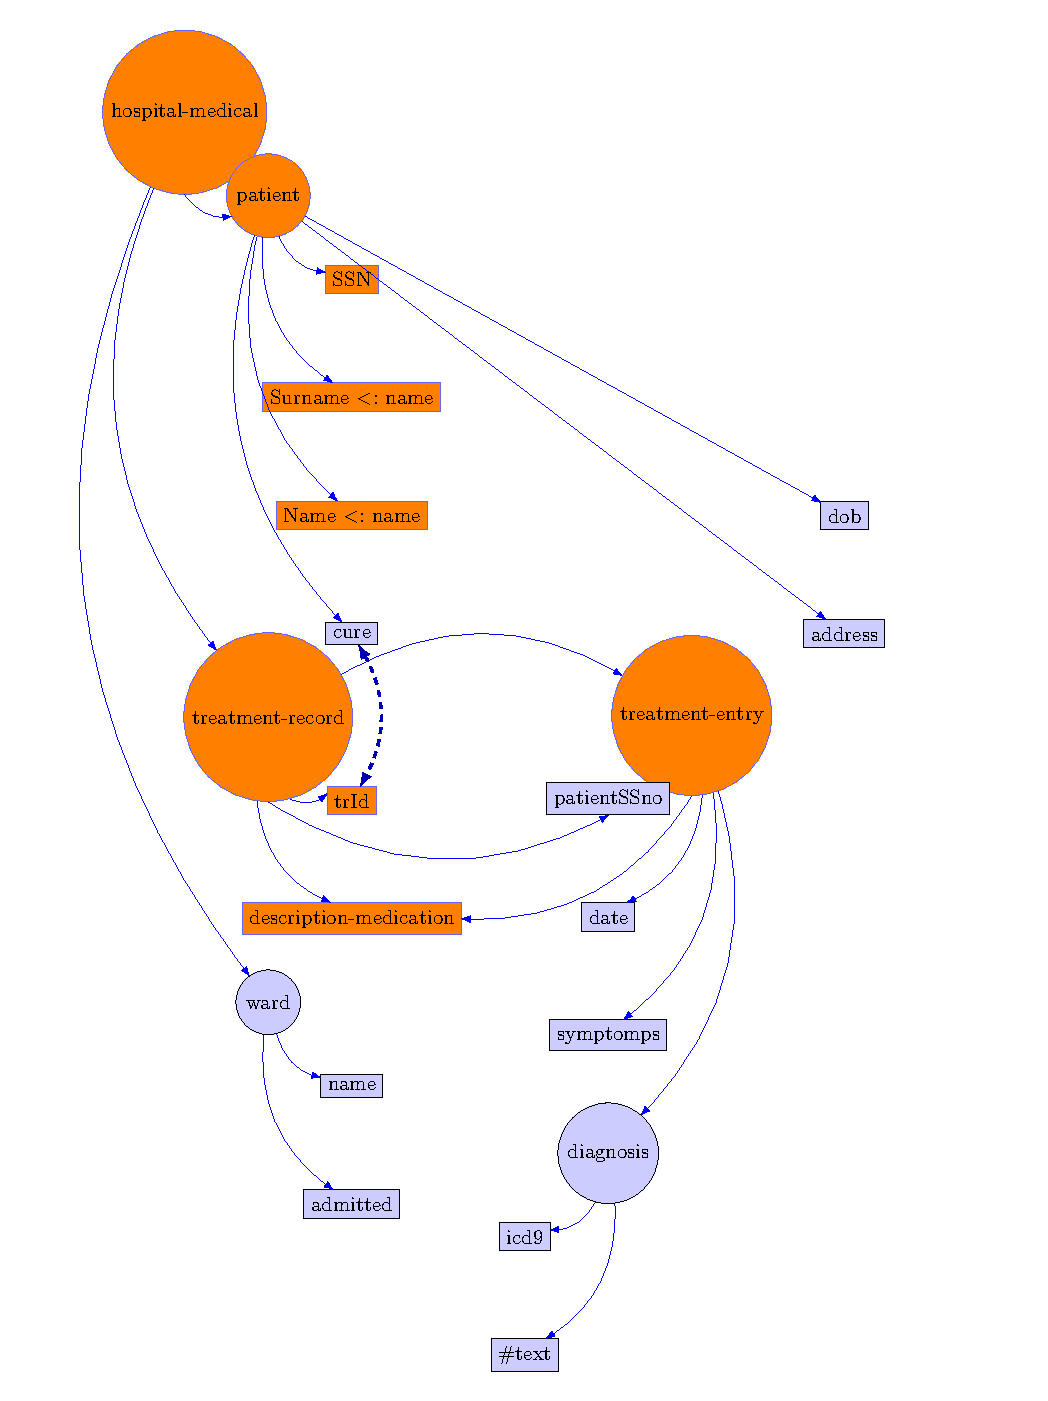
\includegraphics[width=\textwidth]{fig/03joins/ontologyFullJoin}
\caption{Representing an intermediate step for merging the two schemas via providing a graph full join with disjunctive semantics using the green edges as $\theta$ predicates. The vertices showed in orange represent the vertices that have been matched, and hence fused into one single vertex.}
\label{fig:semistructAsMerged}
\end{figure}
\begin{example}
Section \vref{sec:SDIIMRIACR} \index{data integration!schema (graph joins)}introduced the operations of schema alignments between semistructured schemas. Given that literature expresses the containment relations through edges, Figure \vref{fig:semistructAsGraphCont} represents the same structural representation of the former examples in a JSON schema format: now, each vertex represents an empty tuple, where only one single label is associated and therefore showed.

Figure \ref{fig:semistructAsMerged} provides the intermediate result of the schema integration previously provided in Figure \vref{fig:XMLSchemaMergeAfterAlignment}, where multiple matches are not resolved into one single entity (compare the previous \texttt{treatment\_entry} node with the current \texttt{treatment-record} and \texttt{treatment-entry}), where the two schemas where merged using a full join with a disjunctive semantics. This solution allows to preserve the non-matched information, while aggregates together the parts which have been matched within the alignment phase.
\end{example}

%%%%%%%%%%%%%%%%%%%%%%%%%%%
%%%%%%%%%%%%%%%%%%%%%%%%%%%
%%%%%%%%%%%%%%%%%%%%%%%%%%%

\section{Conclusions}
This chapter showed the dualism between \textit{logical model} used to represent data in a formal model and the \textit{physical model}  used for the final algorithms. While the former representation separates the operations on the vertices from the one over the edges, that are run in a subsequent step, the latter allows an implementation of the join algorithm over an adjacency lists combining both vertices and edges within the same step. The inefficiency of the first approach is also showed by the current graph data structures and graph databases, that provide a non scalable implementation of such join algorithms. We can also note that the bucketing phase allows to pre-process the graph in order to enhance the parallelization of the graph join algorithm. Furthermore, given the graph operator's commutative and associative properties, we plan to perform further studies for distributed graph multi-joins in order to check whether current relational query model proposed in \cite{AmelootGKNS17} can be also used for graph data.

Last, it was showed that the graph join operators can be used both to combine data and schema representations; therefore, the graph join acts as a relevant graph operator for data integration at two distinct abstraction levels. Further investigations must be carried out in order to analyse whether it is useful to join graph data with their respective schema.